%-----------------------------------------------------------
%	Model scaling for parameter estimation
%-----------------------------------------------------------
\subsection{Model scaling method to improve parameters correlation for parameter estimation} \label{sec:modelscaling}

%-----------------------------------------------------------
%	Computational approaches	
\subsubsection{Parameter correlation for exponential type models}

	One challenging problem with model parameter determination is covariance between the parameters during parameter estimation. Covariance explains how two parameters influence the response of the model and how they will be updated during parameter estimation. High parameter covariance results in both slow convergence and poor reliability and reproducibility of the material parameters. When scaled by the variance of the two parameters, this becomes the correlation between the parameters, with an absolute value between $0$ and $1$. Correlation equal to $1$ implies that two parameters have the exact same effect on the model response, and are thus indistinguishable during parameter estimation. The covariance issue for constitutive models with an exponential function is well described by Aggarwal \cite{aggarwal_inverse_2015, aggarwal_improved_2017}. These constitutive models with exponential functions have a long valley like region in the objective function space. Inside this valley, significantly different parameters produce similar objective function values. This present several problems. 1) It's difficult to compare model parameters between different specimens, because drastically different parameters can produce similar responses. As such, average or representative specimen has little real meaning, and each specimen needs to be fitted individually for simulations. 2) Once trapped in the valley, the convergence of gradient based optimization algorithms becomes excruciatingly slow due to the small gradients while within this valley. 3) The covariance between parameters are extremely large, decreasing the accuracy or in other word increasing the confidence interval of parameters obtaining. 
    
    Aggarwal \textit{et al.} suggested two improvements to alleviate this problem \cite{aggarwal_improved_2017}. These improvements are 1) modifying the modulus parameter $A$ to $e^{a}$, straightening the shape of the valley, and 2) introduce the log-norm for the objective function, improving the gradient along the valley. These modifications have been shown to be effective. However, this is not always ideal. The logarithmic norm suggested faces some issues when fitting stresses or strains, which may be negative and thus becomes undefined. Although this may be alleviated by forgoing data points with negative strains or stresses, but the model may still produce negative values during parameter estimation. Other methods can be used to discard negative values or to take the norm of such values, but these approaches create discontinuities in the gradient of the objective function, causing convergence problems during parameter estimation. Clearly, additional improvements can still be made. 


%-----------------------------------------------------------
%	Scaling method
\subsubsection{Model scaling method}

	We begin by examining the fundamental reason for the high parameter covariance. For this, we will use the 1-D case as an example,
%==========================================================%
%-------------------	begin EQUATION 	-------------------%
\begin{equation}
\begin{aligned}
\Psi &= A \left(e^{B \epsilon} - 1\right) \\
\mathcal{F} &= \sum_i \left(\Psi(\epsilon_i) - \Psi_i \right)^2,
\end{aligned}
\end{equation}
%-------------------	 end EQUATION 	-------------------%
%==========================================================%
where $\Psi$ is the strain energy of our model, $\epsilon$ is some invariant that is a function of the strain, $\epsilon_i$ and $\Psi_i$ are simulated data, and $\mathcal{F}$ is our objective function for parameter estimation. The parameters $A$ and $B$ have different purposes: $A$ is like a modulus, linearly increasing the stiffness of the material, while $B$ modifies the shape of the response, controlling the nonlinearity of the material. However, practically, the two parameters have nearly the same effect on the mechanical response, increasing $A$ increases the stiffness (Fig. \ref{fig:scalingapproach}A) and increasing $B$ also increases the stiffness (Fig. \ref{fig:scalingapproach}B). This is the reason for the high correlation between the parameters (Fig. \ref{fig:scalingapproach}), 0.9979.


%%%%%%%%%%%%%%%%%%%%%%%%%%%%%%%%%%%%%%%%%%%%%%%%%%%%%%%%%%%%
%-------------------	begin FIGURE 	-------------------%
\begin{figure}
\centering
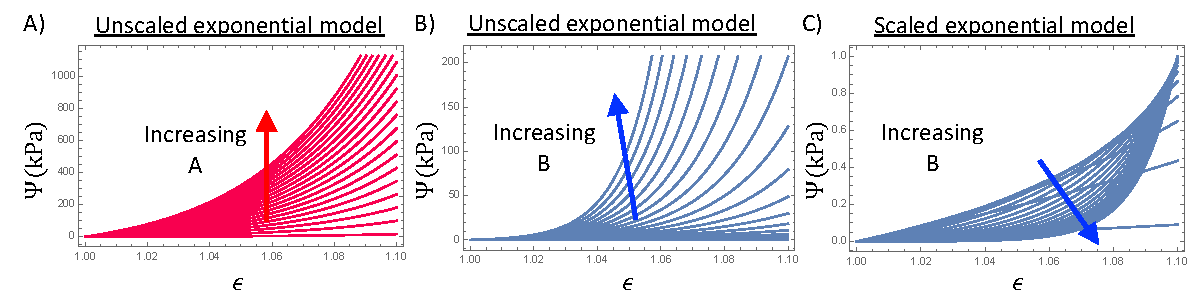
\includegraphics[width=6.5in]{Figures/scalingapproach}
\caption{A)The effect of increasing the values of the modulus $A$ on exponential type models. B) The effect of increasing the values of exponent $B$ on exponential type models, which is very similar to the modulus $A$. C) The effect of increasing the values of parameter $B$ after applying the proposed scaling, increasing the values of parameter $A$ remains the same as in A).}
\label{fig:scalingapproach}
\end{figure}
%-------------------	 end FIGURE 	-------------------%
%%%%%%%%%%%%%%%%%%%%%%%%%%%%%%%%%%%%%%%%%%%%%%%%%%%%%%%%%%%%


	To address this problem, we introduce a scaling term to normalize the exponential part of the model, preventing increasing $B$ from increasing the value of the strain energy as a whole, allowing it to only control the curvature. For this, we will use a value $\epsilon_{max}$, which represents the data point with the maximum strain energy value used for parameter estimation, which is also the point where the strain energy stays the same with changes in $B$. The scaled form is thus given by
%==========================================================%
%-------------------	begin EQUATION 	-------------------%
\begin{equation}
\begin{aligned}
\Psi = \Psi_s = \bar{A} \left[e^{-B\epsilon_{max}} \left( e^{B\epsilon} - 1\right)\right],\label{eqn:scaledmodel1D}
\end{aligned}
\end{equation}
%-------------------	 end EQUATION 	-------------------%
%==========================================================%
where $\bar{A}$ is the scaled version of the modulus $A$. This scaling keeps the exponential part of the model, $e^{-B\epsilon_{max}} ( e^{B\epsilon} - 1)$, at approximately the same value of 1.0 at $\epsilon_{max}$, regardless of the changes in the values of the parameter $B$ (Fig. \ref{fig:scalingapproach}C). This effect is not exact for values of $B < 5$ due to the $-1$ needed to set the strain energy to 0 in the referential configuration, but is nonetheless sufficient for our goal: decoupling the modulus increasing effect of the parameter $A$ from the curvature increasing effect of parameter $B$. Indeed, we found this approach to be successful. We examined the contour plot of the objective function with respect to each of the 4 cases in Aggarwal's work \cite{aggarwal_improved_2017}, with the standard objective function, with $A=e^{a}$, with log-norm, and with $A=e^{a}$ and the log-norm, for both the case without scaling and with scaling (Fig. \ref{fig:objfunctionsurfaces}). First, correlation between the parameters do not change with $A=e^{a}$. The log-norm improves the correlation from 0.9979 to 0.9063(Table \ref{tb:ABcorrelation}), which significantly improves the objective function surface (Fig. \ref{fig:objfunctionsurfaces}). On the other hand, our scaling method improves the correlation from 0.9979 to 0.6186, more significant than using the log-norm. Interestingly, combining scaling and the log-norm has the adverse effect, increasing the correlation back from 0.6186 to 0.8592. This is a result of essentially linearizing the relation between $A$ and $B$, i.e. from $Ae^{B\epsilon}$ to $Log(A)+B\epsilon$, causing the relationship between $A$ and $B$ to go from modulus and nonlinearity to baseline and modulus. Clearly, \emph{the most optimal parameter estimation approach is to use scaling method with no other modifications}. 
    
    
%%%%%%%%%%%%%%%%%%%%%%%%%%%%%%%%%%%%%%%%%%%%%%%%%%%%%%%%%%%%
%-------------------	begin FIGURE 	-------------------%
\begin{figure}
\centering
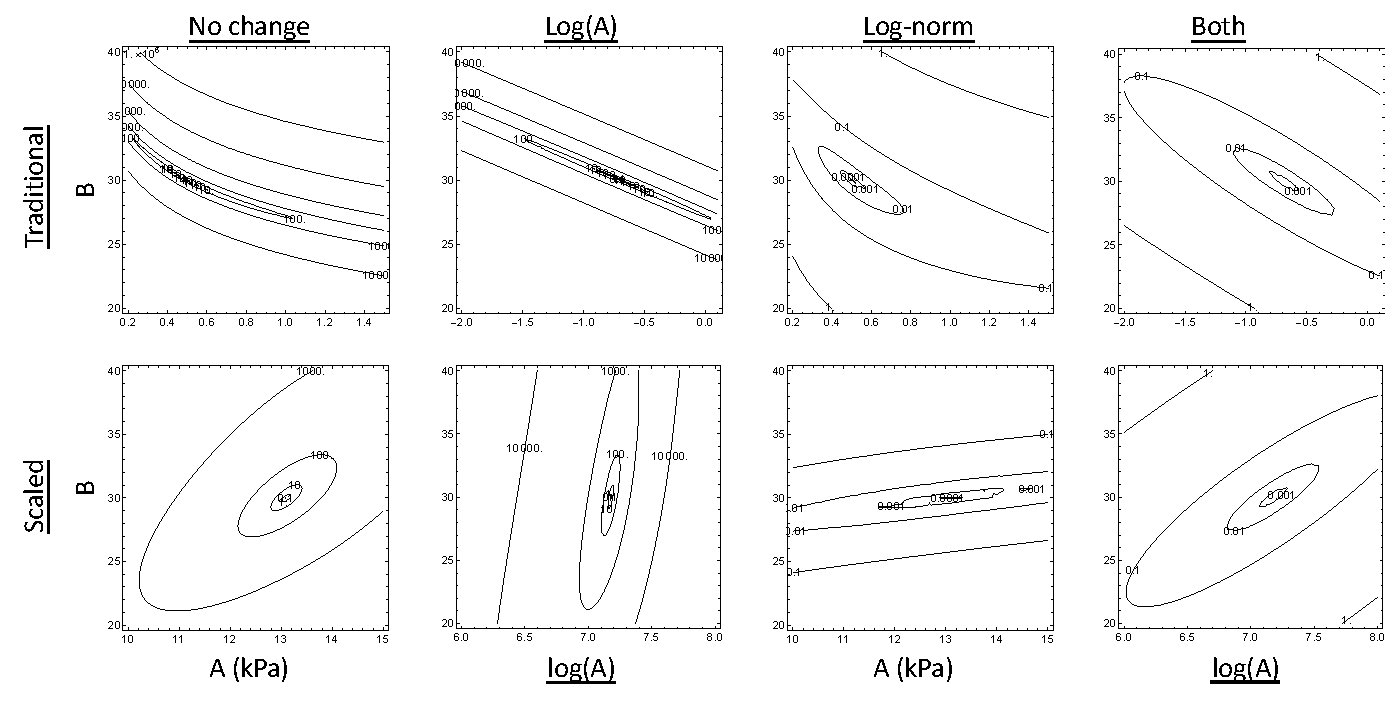
\includegraphics[width=6.5in]{Figures/objfunctionsurfaces}
\caption{(Top) The objective function surface for the traditional unscaled exponential models and (Bottom) objective function surface after scaling. From Left to Right are: the unchanged surface, the surface after changing $A$ to $e^{a}$, using the log-norm for the objective function, and applying both changes. The scaled form with no other changes behaves the best.}
\label{fig:objfunctionsurfaces}
\end{figure} 
%-------------------	 end FIGURE 	-------------------%
%%%%%%%%%%%%%%%%%%%%%%%%%%%%%%%%%%%%%%%%%%%%%%%%%%%%%%%%%%%%


%----------------------------------------------------------%
%-------------------	begin TABLE 	-------------------%
\begin{table}
\caption{The correlation between model parameter when using Hencky strains}
\begin{center}
\label{tb:ABcorrelation}
\begin{tabular}{|l|rrrr|}
\hline
			& No change	& $\log(A)$	& $\log$-norm	& Both \\
\hline
Traditional	& -0.9979	& -0.9979	& -0.9063		& -0.9063 \\
Scaled 		& 0.6186	& 0.6186	& 0.8592		& 0.8592 \\
\hline
\end{tabular}
\end{center}
\end{table}
%-------------------	 end TABLE 		-------------------%
%----------------------------------------------------------%



%-----------------------------------------------------------
%	Relation to unscaled form
% \subsubsection{Relation to unscaled model}

    By design, the value of the exponential parameters $B$ does not change by using the scaling method. Since the scaling term does not depend on the input strain, it acts as a modification to the modulus $A$ while keeping the exponential term the same. This also implies that the relationship between the unscaled modulus $A$ and the scaled modulus $\bar{A}$ is
%==========================================================%
%-------------------	begin EQUATION 	-------------------%
\begin{equation}
\begin{aligned}
A = \bar{A} e^{-B\epsilon_{max}},
\end{aligned}
\end{equation}
%-------------------	 end EQUATION 	-------------------%
%==========================================================%
making finding the actual unscaled parameters a simple task. One other benefit of this scaling approach is that the value of $\bar{A}$ is extremely straight forward and intuitive, it is the strain energy of the model at $\epsilon_{max}$. As a result, the value of $\bar{A}$ can be determined \textit{a priori}, or at the very least very easy to make an initial guess for. This will in turn also help to make parameter estimation faster and more accurate, leaving only the parameter $B$ to be determined. 


%-----------------------------------------------------------
%	Extension to multi-variable form
\subsubsection{Extension to multiple variables}

	Extending this method to multiple variables is very simple. For $\Psi_{eff}$ (Eqn. \ref{eqn:finalmodelform}), the input variables become $\mathbf{\epsilon} = \{E_m, E_n, E_\phi\}$, and $\mathbf{\epsilon}_{max} = \{E_m^{max},E_n^{max},E_\phi^{max}\}$. Determining the values for $\mathbf{\epsilon}_{max}$ depends on the form of the objective function. Using the most common case as the example, which is the sum of the squares of the differences in the 2nd Piola Kirchhoff stress,
%==========================================================%
%-------------------	begin EQUATION 	-------------------%
\begin{equation}
\begin{aligned}
\mathcal{F} = \sum_i \left(S_{11}(\epsilon_i) - \hat{S}_{11}^i\right)^2 + \left(S_{12}(\mathbf{\epsilon}_i) - \hat{S}_{12}^i\right)^2 + \left(S_{22}(\epsilon_i) - \hat{S}_{22}^i\right)^2,
\end{aligned}
\end{equation}
%-------------------	 end EQUATION 	-------------------%
%==========================================================%
$\mathbf{\epsilon}_{max}$ is the data point $\mathbf{\epsilon}_i$ which maximizes $\left(\hat{S}_{11}^i\right)^2 + \left(\hat{S}_{12}^i\right)^2 + \left(\hat{S}_{22}^i\right)^2$. 
Thus, we also introduce a $Q_{max}$ such that,
%==========================================================%
%-------------------	begin EQUATION 	-------------------%
\begin{equation} \label{eqn:finalexponentialmodelformscaled}
\begin{aligned}
\Psi_{eff} 	=& c_0 \left(e^{Q} - 1\right) + \Psi_\mathrm{mat} - p\left(\mathrm{J}-1\right) \\
            =& c_0^\prime e^{-Q_{max}}\left(e^{Q} - 1\right)	
	+ \frac{\eta_M}{2} \left( \frac{1}{\alpha}\left( I_1 -3\right)^{\alpha} + \frac{r}{\beta} \left( I_1 -3\right)^{\beta} \right) - p\left(\mathrm{J}-1\right)\\
Q		=& b_1 E_m^2 + b_2 E_n^2 + b_4 E_m E_n + b_5 E_m^4 + b_6 E_n^4 +
b_9 E_m E_m^3 + b_{10} E_n^4 + b_{11} E_m^2E_\phi^2 + b_{12} E_n^2 E_\phi^2 	\\
Q_{max}	=& b_1 (E_m^{max})^2 + b_2 (E_n^{max})^2 + b_4 E_m^{max} E_n^{max} + b_5 (E_m^{max})^4 + b_6 (E_n^{max})^4 +
b_9 E_m^{max} (E_m^{max})^3 	\\
		&+ b_{10} (E_n^{max})^4 + b_{11} (E_m^{max})^2(E_\phi^{max})^2 + b_{12} (E_n^{max})^2 (E_\phi^{max})^2,
\end{aligned}
\end{equation}
%-------------------	 end EQUATION 	-------------------%
%==========================================================%
where parameter estimation will be done for $c_0^\prime$ instead of $c_0$. Computing the response functions and the stresses, or even the elasticity tensor remains very simple, only requiring multiplying each term by $e^{-Q_{max}}$. Thus, this scaling method is a very simple and easy to implement method of improving the speed and convergence for the parameter estimation of exponential type models. 



